\documentclass[10pt,twocolumn,letterpaper]{article}

\usepackage{iccv}
\usepackage{times}
\usepackage{epsfig}
\usepackage{graphicx}
\usepackage{amsmath}
\usepackage{amssymb}

% Include other packages here, before hyperref.

% If you comment hyperref and then uncomment it, you should delete
% egpaper.aux before re-running latex.  (Or just hit 'q' on the first latex
% run, let it finish, and you should be clear).
\usepackage[breaklinks=true,bookmarks=false]{hyperref}

\iccvfinalcopy % *** Uncomment this line for the final submission

\def\iccvPaperID{****} % *** Enter the ICCV Paper ID here
\def\httilde{\mbox{\tt\raisebox{-.5ex}{\symbol{126}}}}

% Pages are numbered in submission mode, and unnumbered in camera-ready
%\ificcvfinal\pagestyle{empty}\fi
\setcounter{page}{1}
\begin{document}

%%%%%%%%% TITLE
\title
{
    Classification of Histology and Pathology Images Using Convolutional Neural
    Networks%
}

\author{%
    Luong Nguyen\\
    University of Pittsburgh\\
    Biomedical Building Tower 3\\
    Fifth Ave\\
    Pittsburgh, PA 15026\\
    {\tt\small luongn@andrew.cmu.edu}
    \and
    Dan Spagnolo\\
    University of Pittsburgh\\
    Biomedical Building Tower 3\\
    Fifth Ave\\
    Pittsburgh, PA 15026\\
    % {\tt\small luongn@andrew.cmu.edu}
    \and
    Jakob Bauer\\
    Carnegie Mellon University\\
    5000 Forbes Avenue\\
    Pittsburgh, PA 15213\\
    {\tt\small jsbauer@andrew.cmu.edu}
}

\maketitle
%\thispagestyle{empty}


%%%%%%%%% ABSTRACT
% \begin{abstract}
%    The ABSTRACT is to be in fully-justified italicized text, at the top
%    of the left-hand column, below the author and affiliation
%    information. Use the word ``Abstract'' as the title, in 12-point
%    Times, boldface type, centered relative to the column, initially
%    capitalized. The abstract is to be in 10-point, single-spaced type.
%    Leave two blank lines after the Abstract, then begin the main text.
%    Look at previous ICCV abstracts to get a feel for style and length.
% \end{abstract}

%%%%%%%%% BODY TEXT

\section{Introcuction}
\label{sec:Introcuction}

Deep learning has accomplished multiple successes with natural images,
including segmenting, tagging, and scene understanding. However, only
recently has deep learning ventured into the realm of medical images with
multiple papers appeared in the top-tiered conference in medical imaging
[1] [2]. The slower adaptation of deep learning in medical image analysis
could be explained by several limitations of this field, including expensive
image capture, cost prohibitive annotations, and the lack of publicly
available datasets with annotations. It takes eight years to train a
pathologist and one year is spent on learning histology (i.e., recognizing
images of normal tissues from different organs). This motivates us to build
an automated system to classify tissues from different organs.

\section{Aims}
\label{sec:Aims}

Facing these challenges, our team sets out to answer the following questions
on learning from these images: (1) Can we train a convolutional neural network
(CNN) to differentiate normal tissues from different organs? If so, what are
the differentiating features of tissues? (2) Can we train a CNN to
differentiate between normal and cancerous tissues from the same organs?
If so, what are the differentiating features? (3) Can we train a CNN to
differentiate cancerous tissues from different organs? If so, what are the
differentiating features? (4) can we improve our classifier to a significant
degree using augmentation methods to increase our training data? If our CNN
could not achieve any of the above goals, even with data augmentation, where
did we go wrong?

\section{Dataset}
\label{sec:Dataset}

We curated a set of 69 whole slide images (WSIs) of tissues from 25 different
organs. They are microscope images of hematoxylin and eosin (H\&E stained)
tissues in which H stains nuclei purple and E stains cytoplasm and connective
tissue pink. The WSIs were collected from UPMC Shadyside and scanned using
Aperio XT scanner. Each WSI is of size 20,000 x 30,000 pixels at 20x
magnification. These images will be divided into overlapping patches of size
256 x 256 pixels and only patches with tissues (non-empty space) are included
in the analysis, resulting in about 4000 patches/WSI. In addition, for each
organ, we will download 2 WSIs from the publicly available Cancer Genome Atlas
(TCGA) to answer the questions related to cancerous tissues.

\section{Methods}
\label{sec:Methods}

We will try multiple methods for data augmentations to increase the number of
patches per WSI up to 10000 patches. These methods may include rotating and
flipping patches, scale jittering, modifying color and brightness, as well as
adding noise to patches [3]. In addition to ground truth, we will collect
non-expert naive observer (Jakob)’s and intermediate observer (Daniel)’s
annotations for comparison with human classification. For baseline comparison
with shallow learning methods, we can train an SVM with SIFT/HOG features [4].
We will experiment with standard CNN architectures such as AlexNet, VGGNet,
and LeNet. We suspect that our problem will not require as many CNN layers
as 1000-class datasets, for example, and thus we will experiment with CNN
depth. We will use Torch or Caffe to train our CNNs. The last layer will be
removed to generate feature vectors. These feature vectors will serve as
input to a classifier (SVM, logistic regression) to determine the tissue
origin and disease status. Finally we will conduct error analysis to find
out where we can improve our CNN. The metrics for comparisons will be
precision-recall curves and F1 scores. Our goal is to outperform our shallow
learning baseline as well as our naive and intermediate observers.

\section{Expected Complications}
\label{sec:Expected Complications}

From our experience with classes in histology, it is possible to train a human
to accomplish aim (1) fairly well after a one-semester class (Luong and Dan
took a histology class). The ability to differentiate normal tissues from
different organs is based on recognizing landmark features of different
organs. For examples, kidney tissues have outer and inner cortex while breast
tissues have clusters of milk conducting ducts (see
Figure 1, left).
Therefore, we are convinced that it is plausible to teach computers to read
normal histology images. However, patches taken from WSI do not always
contain landmark features of organs and tissue types. For example, adipose
(fat) tissue is the same for many organs. We may not be able to properly
classify image patches if these landmark features are not sampled in a given
patch. This implies high false positive rate if we try to classify patches
into different tissues. In addition, we might encounter difficulties analyzing
cancerous tissues since invasive cancer can completely destroy the unique
structures of different tissue types. Therefore, we expect to have a hard
time accomplishing the task in aim (3) since destroyed tissue structures can
look very similar across different organs. Another complication can come from
the color variation of these tissue images since different hospitals and
pathologists have different slide preparation procedures. This means the
CNN can focus on figuring out different color schemes for classification
instead of actually discovering different structures of tissues. To resolve
this, we will apply some standard color normalization for histology images.

Finally, there is some concern for the number of training and testing images
we will have. Due to the cost of data acquisition in this domain, our dataset
scale is much smaller than would be found in typical datasets in the computer
vision field. We will attempt to overcome this difficulty using the data
augmentation techniques described in Methods. If our shallow learning
methods outperform the deep learning approach, this may be indicative of
insufficient data.

\begin{figure}[h]
\begin{center}
% \fbox{\rule{0pt}{2in} \rule{0.9\linewidth}{0pt}}
   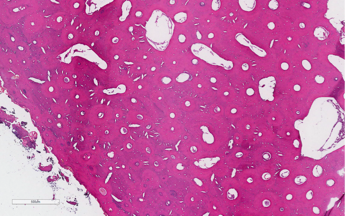
\includegraphics[width=0.9\linewidth]{figures/image00.png}
\end{center}
    \caption
    {%
        Breast tissue with ducts and lobules.
    }
\label{fig:long}
\label{fig:onecol}
\end{figure}

\begin{figure}[h]
\begin{center}
% \fbox{\rule{0pt}{2in} \rule{0.9\linewidth}{0pt}}
   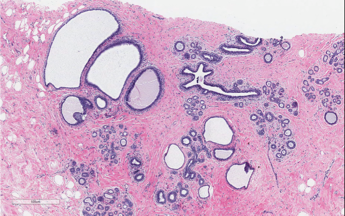
\includegraphics[width=0.9\linewidth]{figures/image01.png}
\end{center}
    \caption
    {%
        Bone tissue with large area of pink stained calcium.
    }
\label{fig:long}
\label{fig:onecol}
\end{figure}

% \begin{figure*}
% \begin{center}
% \fbox{\rule{0pt}{2in} \rule{.9\linewidth}{0pt}}
% \end{center}
%    \caption{Example of a short caption, which should be centered.}
% \label{fig:short}
% \end{figure*}

% For this citation style, keep multiple citations in numerical (not
% chronological) order, so prefer \cite{Alpher03,Alpher02,Authors14} to
% \cite{Alpher02,Alpher03,Authors14}.
%
% When placing figures in \LaTeX, it's almost always best to use
% \verb+\includegraphics+, and to specify the  figure width as a multiple of
% the line width as in the example below
% {\small\begin{verbatim}
%    \usepackage[dvips]{graphicx} ...
%    \includegraphics[width=0.8\linewidth]
%                    {myfile.eps}
% \end{verbatim}
% }

%------------------------------------------------------------------------

\section{References}
\label{sec:References}

%-------------------------------------------------------------------------

{\small
\bibliographystyle{ieee}
\bibliography{egbib}
}

\end{document}
